\section{Objektorientierte Anfragen und Implementierungskonzepte}

\subsection{Objektorientierte Anfragesprachen: Kriterien und Grundlagen}
\begin{itemize}
	\item allgemeine Prinzipien SQL-artiger Anfragesprachen
	\item OO Konzepte (Typkonstruktoren, Komponentenobjekte, Vererbung, Methodenaufrufe,..) unterstützen
	\item möglichst kompatibel zum Standard-SQL (???)
	\item relationale, objekterzeugende (?) und objekterhaltende (???) Semantik
	\item Kriterien für Anfragesprachen erfüllen
	
	\item \textbf{Kriterien Anfragesprachen}
	\begin{table}[!h]
		\centering
		\begin{tabular}{|l|p{20em}|c|c|}
			\hline
			\textbf{Kriterium}	& \textbf{Erklärung} & \textbf{Manifesto} & \textbf{OQL}\\
			\hline
			\hline
			Deskriptive Sprache & Die Sprache soll nicht navigierend sein, einen Zugriff auf eine Menge von Objekten ermöglichen & \checkmark & \checkmark\\
			\hline
			Optimierbarkeit & Die Sprache soll nach (etwa algebraischen) Regelsystemen konzeptuell optimierbar sein & \checkmark & \checkmark\\
			\hline
			Effizienz & Die wenigen Grundoperationen sollen mit einer geringen Komplexität implementierbar sein. & \checkmark & \checkmark\\
			\hline
			Orthogonalität & Die beliebigen Grundoperationen sollen beliebig miteinander kombinierbar sein. & $\circ$ & \checkmark\\
			\hline
			Erweiterbarkeit & Bei Erweiterung des OODMs soll auch die SPrache leicht erweiterbar sein. & $\circ$ & $\circ$\\
			\hline
			Abgeschlossenheit & Das Ergebnis jeder Anfrageoperation soll wieder konsistent im Strukturteil des Datenbankmodells darstellbar sein. & $\circ$ & \checkmark\\
			\hline
			Adäquatheit & Alle Konstrukte des Datenbankmodells sollen ausgenutzt werden, für alle Strukturen muss es Anfrageoperationen geben. & $\circ$ & $\circ$\\
			\hline
			Sicherheit & Jede Anfrage soll ein endliches Ergebnis liefern. & $\circ$ & $\circ$\\
			\hline
			Vollständigkeit & Es soll zumindest die Mächtigkeit relationaler Anfragesprachen erreicht werden. & \checkmark & \checkmark\\
			\hline
			Formale Semantik & Die Operationen der Sprache sollen formal definiert sein. & $\circ$ & \checkmark\\
			\hline
		\end{tabular}
	\end{table}
	
	\item \textbf{Einschub: Generische Update-Operationen}
	\begin{itemize}
		\item generische Updates (5 Typen statt 3 relational)
		\item Updates auf Extension einer Klasse:
		\begin{itemize}
			\item Erzeugen mit create oder new (in abstrakter Klasse)
			\item Löschen mit forget, destroy oder delete (in abstrakter Klasse)
			\item Einfügen mit insert, add oder gain in Objektmenge einer anderen (freien) Klasse
			\item Herausnehmen mit remove oder lose aus Objektmenger einer (freien) Klasse
		\end{itemize}
		\item Updates auf Zuständen (Tupel, Mengen, Listen, Standard-Datentypen)
	\end{itemize}
	
	\item \textbf{Relationale Operationen}
	\begin{itemize}
		\item Algebren für Relationen mit Typkonstruktoren
		\item Minimale geschachtelte Algebra
		\item Orthogonale geschachtelte Algebra
		\item Algebren für spezielle geschachtelte Relationen: PNF-Algebra\\
		PNF geeignet als ALgebra für Objektrelationen: Sicherung der Eindeutigkeit der Objektidentität auch im Ergebnis (Grundlage für objekterhaltende Anfragen)
		\item Instanz einer Klasse: Objektrelation
		\item jetzt: Objektrelation als geschachtelte Relation auffassen:\\
		Ergebnis einer Anfrage: geschachtelte Relation, nicht Objektrelation\\
		Eingabe: Klassen in Klassenhierarchie mit komplexen Zustandstypen\\
		AUsgabe: Elemente (Werte) eines komplexen Typs
		\item Operationen:\\
		Relationenalgebra und NEstung, Entnestung (minimal)\\
		jede Relationenalgebra-Operation homogen erweitert (orthogonal)
	\end{itemize}
	
	\item \textbf{Minimale geschachtelte Algebra}
	\begin{itemize}
		\item Projektion, Selektion (evtl Bedingungen auch an Collections), Verbund, Mengenoperationen und Umbenennung aus Relationenalgebra; zusätzlich:
		\item \textit{Nestung:} Eine Nestung $v[(A_1, \ldots, A_n);A](r(R))$ fasst die Attribute $A_1, \ldots, A_n$ des Relationenschemas $R$ zu einen neuen Attribut $A$ zusammen, d.h. $A$ ist definiert als $set(tuple(A_1, \ldots, A_n))$. Mehrere $(A_!, \ldots, A_n)$-Tupel werden zu einer Menge zusammengefasst, wenn die Werte der Tupel in der Relation $r$ auf den restlichen Attributen des Relationenschemas (also auf $R - \{A_1, \ldots, A_n\})$ übereinstimmen.
		
		\item \textit{Entnestung:} Eine Entnestung $\mu[A](r(R))$ löst das Nest $A$ auf, d.h. falls $A$ als $set(tuple(A_1, \ldots, A_n))$ definiert ist, sind im Ergebnis die Attribute $A_1, \ldots, A_n$ im Relationenschema enthalten. Die Einzelnen Tupel der Attributwerte von $A$ werden zusammen mit den zugehörigen Attributwerten der restlichen Attribute von $R$ zu neuen Tupeln verbunden.
		
		\item Entnestung mach Nestung rückgängig; Umkehrung gilt nicht immer
		\item minimale Algebra umständlich: meist Entnestung, Operationen, Nestung
		\item Bsp: siehe VL Folien 5-8 bis 5-11
	\end{itemize}
	
	\item \textbf{Orthogonale geschachtelte Algebra}
	\begin{itemize}
		\item Bsp: Algebra von Schek und Scholl
		\item Projektion und Selektion werden rekursiv:\\
		Projektion, Selektion in Projektionsliste\\
		Projektion, Selektion in Selektionsbedingung
		\item Bsp: Innerhalb der Projektionsliste das komplexe Attribut \textit{Belegschaft} auf das in ihm enthaltene Attribut \textit{Nachname} projizieren:
		\[\pi [Institut, \pi[Nachname](Belegschaft)](r') \]
		\item jede bel. Kombination (P - Projektion, S - Selektion: P in P, P in S, S in P, S in S) erlaubt
		\item auch Prädikate auf Collections: $\subset, \in$
	\end{itemize}
	
	\item \textbf{ALgebren für spezielle geschachtelte Relationen}
	\begin{itemize}
		\item statt Objektrelationen $\to$ geschachtelte Relation
		\item jetzt Objektrelation $\to$ Objektrelationen
		\item Algebra auf PNF-Relation (Partitioned Normal Form; müssen PNF-Eigenschaft erhalten)
		\item Projektion muss flachen Schlüssel bewahren (flach: 1NF; Attribut vom Std-Typ)
		\item Verbund muss gerichtet sein ((Typ-)Erweiterung statt Verbund)
		\item Vereinigung wird rekursiv
	\end{itemize}
	
	\item \textbf{Eigenschaften von PNF-Relationen}
	\begin{itemize}
		\item Bsp: $r'$ ist PNF-Relation, da auf jeder der drei Ebenen ein flaches Attribut Schlüssel ist
		\item PNF-Relationen können immer durch vollständige Entnestung als flache Relationen dargestellt werden und ohne Verlust von Informationen zur ursprünglichen PNF-Relatoin zurückgenestet werden
		\item Konsequenz: PNF-Relationen vermeiden das Problem der ersten Übungsaufgabe
		\item PNF-Relationen entsprechen auf der ersten Stufe der Semantik von Objektrelationen: Objektidentität muss für Objektrelation Schlüssel sein
	\end{itemize}
	\item \textbf{Fazit} Algebren für geschachtelte Relationen\\
	Orthogonale Algebra: gute Basis für relationale Anfragen an Objektrelationen\\
	PNF-Algebra: gute Basis für objekterhaltende Anfragen an Objektrelationen
\end{itemize}


\subsection{Beyond OQL: Objekterzeugende und objekterhaltende Anfragen}
\begin{itemize}
	\item \textbf{Objekterzeugende Operationen:}\\
	\begin{itemize}
		\item \textbf{implizites Erzeugen}
		\begin{itemize}
			\item Erzeugung nicht steuerbar und nicht sichtbar
			\item jede Operation, jede Anfrage objekterzeugend
			\item Bsp: Selektion nach Rostocker Studenten erzeugt neue Klasse von Objekten, die aber keine Studenten mehr sind
		\end{itemize}
		\item \textbf{freies Erzeugen}
		\begin{itemize}
			\item Erzeugung steuerbar und sichtbar
			\item einige Operationen beinhalten Kennung zur Erzeugung von Objekten
			\item NAchteil: Prozess kann in rekursiven Anfragen nicht kontrolliert werden
		\end{itemize}
		\item \textbf{Objekterzeugende Funktionen} (insb. bei Rekursion nötig)
		\begin{itemize}
			\item bei Erzeugung wird angegegebn, zu welchen Werten Objektidentitäten erzeugt werden
			\item Erzeugung ist Funktion, daher in Rekursion zu kontrollieren
		\end{itemize}
	\end{itemize}
	
	\item \textbf{Objekterhaltende Operationen:}
	\begin{itemize}
		\item \textbf{Auflösung von Inkonsistenzen}		\begin{itemize}
			\item Problem nicht nur bei Entnestung (Änderung von Zustandstypen), sondern Objekte mit lokalen Zuständen in Objektrelationen\\
			Beispiel:
			\begin{itemize}
				\item Angestellter $\gamma_{12}$ hat Komponentenobjekt Verantwortlicher $\gamma_{19}$
				\item Person $\gamma_{12}$ hat Komponentenobjekt Verantwortlicher $\gamma_{33}$
				\item nach Vereinigung von Angestellten und Personen setzt sich speziellerer Zustand ($\gamma_{19}$) durch (Overriding)
				\item Aber Problem: Konflikte in unvergleichbaren Klassen
				\item Angestellter $\gamma_{12}$ hat Komponentenobjekt Verantwortlicher $\gamma_{19}$
				\item Student $\gamma_{12}$ hat Komponentenobjekt Verantwortlicher $\gamma_{14}$
				\item Nach Vereinigung von Angestellten und Studenten Konflikt zwischen zwei Verantwortlichen, kein Overriding mgl
			\end{itemize}
			\begin{figure}[!h]
				\centering
				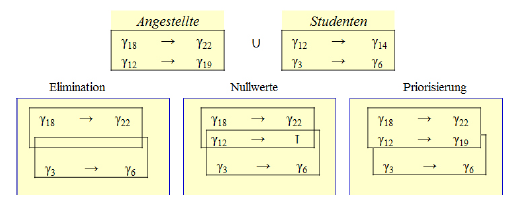
\includegraphics[scale=0.70]{img/resolve_inconsistency.png}
			\end{figure}
			\item Auflösetechnik:
			\begin{itemize}
				\item Elimination (Living in a Lattice)
				\item Nullwerte (F-Logic)
				\item Priorisierung (IQL)
			\end{itemize}
		\end{itemize} 
		\item \textbf{ statische/dynamische Typen} (statisch: extensionsbasierte Anfragen) und \\
		\textbf{statische/dynamische Klassifizierung} (statisch: extensionsbasierte Anfragen)
		\begin{itemize}
			\item Statische Typen:\\
			neue Objektmengen (Extensionen) zusammenstellen, aber Typen können nicht verändert werden\\
			etwa in ODMG-OQL
			\item Dynamische Typen\\
			Zustandstypen können eingeschränkt, erweitert, umstrukturiert werden\\
			Typinferenz in Programmiersprachen; ist relativ einfach lösbar
			\item dynamische Klassifizierung\\
			genaue Einordnung in die Klassenhierarchie unabhängig von aktueller Instanz\\
			im allgemeinen unentscheidbar
		\end{itemize}
		
		Beispiel: Probleme dynamische Klassifizierung
		\begin{itemize}
			\item Wie muss ich folgende Anfrageergebnisse in der Klassenhierarchie einordnen?
			\item $Q_1$: Selektion nach 'Fußball' IN Hobbies;\\
			$Q_2$: Selektion nach 'Tennis' IN Hobbies;
			\item unter Personen, nebeneinander
			\item aber nicht, wenn Integritätsbedingung gilt: alle Fußballspieler müssen auch Tennisspieler sein
			\item dann Ergebnis von $Q_1$ Unterklasse vom Ergebnis $Q_2$
			\item $Q_3$: Selektion nach Alter = 19\\
			$Q_4$: Selektion nach Alter > 17 AND ALter < 19
			\item $Q_3$ und $Q_4$ liefern dieselbe Ergebnisklasse
			\item falls Alter vom Typ integer
			\item nicht bei Typ Real, Float, Decimal, dann $Q_4$ Oberklasse von $Q_3$
			\item $Q_5$ Selektion nach Methode Schlumpf = true\\
			$Q_6$ Selektion nach Methode Schlampf = true
			\item unentscheidbar, falls Methodenimplementierungssprache turing-vollständig
		\end{itemize}
	\end{itemize}
	
\end{itemize}


\subsection{Client-Server-Architekturen von OODBMS}
\begin{figure}[!h]
	\centering
	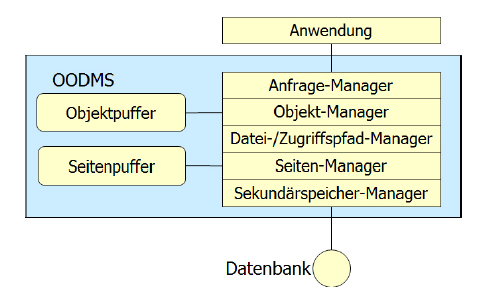
\includegraphics[scale=0.7]{img/client_server_oodbms.png}
	\caption{Client-Server-Architektur von OODBMS}
\end{figure}

\begin{itemize}
	\item modifizierte Fünf-Schichten-Architektur (Objekt-Manager und Objektpuffer zusätzlich)
	\begin{itemize}
		\item Sekundärspeicher-Manager: Verwaltung des Sekundärspeichers, Transport von Seiten in den Hauptspeicher
		\item Seiten-Manager: verwaltete Seitenpuffer und Sperren (von Seiten)
		\item Datei/Zugriffspfad-Manager: Objektidentitäten der Objekte in Seitenadressen umrechnen
		\item Objekt-Manager
		\begin{itemize}
			\item Seitenstrukturen in Objektstrukturen umwandeln, Komponentenbeziehungen und Vererbungsbeziehungen materialisieren
			\item falls duales Pufferkonzept: Objektstrukturen auch im eigenen Objektpuffer verwalten
			\item  Objektidentitäten generieren und verwalten
			\item SPerren auf Objektebene verwalten
		\end{itemize}
		\item Anfrage-Manager oft in OODBS nicht vorhanden, sondern in Anwendungs-Client integriert
	\end{itemize}
\end{itemize}

\begin{figure}[!h]
	\centering
	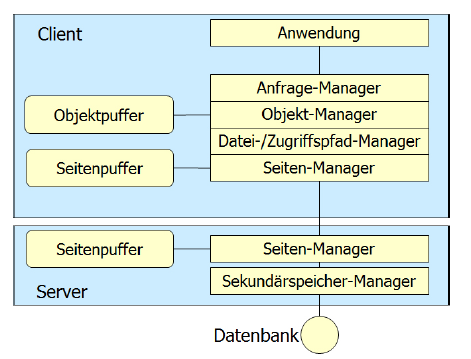
\includegraphics[scale=0.6]{img/seiten_server.png}
	\caption{Seiten Server}
\end{figure}

\begin{figure}[!h]
	\centering
	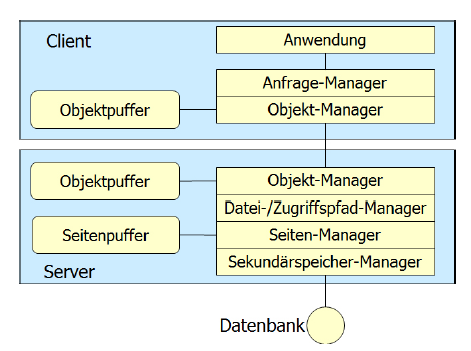
\includegraphics[scale=0.6]{img/object_server.png}
	\caption{Objekt Server}
\end{figure}

\begin{figure}[!h]
	\centering
	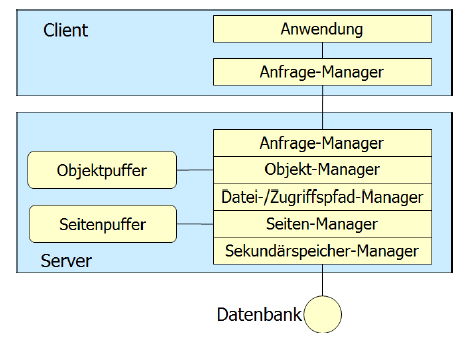
\includegraphics[scale=0.6]{img/anfrage_server.png}
	\caption{Anfrage Server}
\end{figure}

\newpage
\subsection{Persistenz}
\begin{framed}
	\textbf{Definition von Atkinson}
	\begin{description}
		\item Fähigkeit der Daten (Werte oder Objekte), beliebige Lebensdauern (so kurz wie möglich oder so lang wie nötig) anzunehmen, dazu die folgenden Prinzipien einhalten
		\item Typ-Orthogonalität: Daten bel. (auch komplexer) Typen sollen persistent gemacht werden können.
		\item Unabhängigkeit der Programme von der Persistenz: Programm sollen unverändert bleiben, wenn die Daten ihre Lebensdauer ändern.
		\item Persistenzfortpflanzung:\\
		zusammengesetztes Objekt persisten => auch seine Komponentenobjekte\\
		Collection-wertiges Objekt persistent => auch alle Elemente der Collection
	\end{description}
\end{framed}

\begin{itemize}
	\item Punkt 3 schließt so etwas wie MOVE- oder COPY-Befehle aus
	\item Zweistufige Persistenz:\\
	Daten transient: Lebensdauer endet am Block-, Prozedur-, oder Programm-Ende\\
	Daten persistent: Programmende, Systemabstürze, Plattenfehler überleben
	
	\item \textbf{Persistenzmodelle}
	\begin{itemize}
		\item automatische Persistenzfähigkeit 
		\item Persistenzfähigkeit durch Vererbung
		\item Persistenzfähigkeit explizit
	\end{itemize}
	
	\item \textbf{Persistentmachung}
	\begin{itemize}
		\item Bei Erzeugung (pnew oder persistent new) in ODMG: new überladen (new ist transient, new (DB) ist persistent)
		\item durch spezielle Funktionen (Methode persist)
		\item Durch Namensvergabe
	\end{itemize}
	\item \textbf{Persistenzfortpflanzung}
	\begin{itemize}
		\item explizit
		\item durch Erreichbarkeit; Wurzelobjekte oder DB-Einsteigspunkte
	\end{itemize}
	
	\item \textbf{Objektrelationale Persistenz}
	\begin{itemize}
		\item alle Tupel persistent
		\item Persistentmachung durch insert
		\item keine Persistenz durch Erreichbarkeit
	\end{itemize}
\end{itemize}


\subsection{Interne Ebene}
\begin{itemize}
	\item Implementierung von 
	\begin{itemize}
		\item \textbf{Objektidentitäten}
		\begin{itemize}
			\item Darstellung der Objektidentität durch Surrogate und ihre Implementierung durch indirekte Referenzen:
			\item Technik logisch sauberer, aber langsamer
			\item SUrrogate immer eindeutig, auch nach der Löschung des Objektes
			\item in verteilter Umgebung eindeutig (Codierung der Rechner-ID im Surrogate)
			\item abstrakte Klasse, in der das Objekt erzeugt wird, im Surrotgate kenntlich machen
			\item Darstellung und Implementierung der Objektidentität durch direkte Referenzen
			\item Länge: 32 oder 64 Bit
		\end{itemize}
		\item \textbf{Klassen}\\
		{\tiny (ohne komplexe Attributwerte, Komponentenobjekte)}
		\begin{itemize}
			\item Binäre Speicherung: Objekte zusammen mit jeweils einem Attribut als binäre Relation
			\item Objektstruktur mit integriertem Schema:\\
			Schemainformationen in die Speicherstruktur jedes Objekts etwa in ORION/ITASCA; siehe auch XML im 2. Teil der VL
			\item Objektstruktur mit externem Schema\\
			wie in RDBMS/ORDBMS
		\end{itemize}
		\item \textbf{Komplexen Attributen und Komponentenhierarchien...}
		\begin{itemize}
			\item Objekt größer als Seite => mehrere Seiten in Form eines B-Baums
			\item Menge von Objekten einer Klasse geclustert
			\item komplexe Attribute:\\
			zerlegte Speicherung (wie in RDBS normalisiert)\\
			gesamte Objektstruktur in einem Cluster
			\item private Komponentenobjekte: Cluster mgl
			\item gemeinsame Komponentenobjekte: Referenzen auf Komponentenobjekt
		\end{itemize}
		\item \textbf{... evtl. durch Cluster}
		\begin{itemize}
			\item Cluster-Definition zur Zeit der\\
			Klassendefinition (im Schema): O$_2$\\
			Objektinstantiierung (pro Objekt)
			\item Cluster-Strukturen für:
			\item alle Objekte einer Klasse
			\item bestimmte Teile von Klassen, etwa Partition der Klasse nach bestimmten Attributwerten
			\item alle Instanzen von Klassen, die zu einem spezifizierten Teil der Klassenhierarchie gehören (ORION)
			\item zusammengesetzte Objektes (Objekt mit privaten Komponentenobjekten)
			\item komplexe Attributwerte
		\end{itemize}
		\item \textbf{Klassenhierarchien}
		\begin{itemize}
			\item Objekt nur in genau einer Klassen\\
			Zustand dieses Objektes in dieser Klasse gespeichert (Home Class Model) (bei OODBPLs und einigen Neuentwicklungen wie ORION)
			\item Objekt in mehreren Klassen:
			\item Objekt in kleinster Klasse, zusammen mit vererbten Attributwerten (Leaf Overlap Model)
			\item Objekt in jeder Klasse, zusammen mit lokalen Attributwerten (Split Instance Model)
			\item Objekt in jeder Klasse, zusammen mit dort definierten und allen vererbten Attributwerten (Repeat CLass Model) (tiefe Extension direkt)
			\item Alle Objekte in einer Datei, nicht anwendbare Attribute auf null (Universal Class Model)
			\item Alle Objekte in einer ternären Datei mit Surrogate,Attribut und Attributwerte (Value Triple Model)
		\end{itemize}
	\end{itemize}
	
	\item Zugriffspfade für
	\begin{itemize}
		\item \textbf{Klassen}
		\begin{itemize}
			\item grundlegende Dateiorgansiationsform durch Speicherstruktur der Klasse bereits festgelegt
			\item durch Hash-Funktion oder B-Bäume zusätzlich unterstützen
			\item Zugriff auf Objekte in Klassenhierarchien und Komponentenhierarchien unterstützen
			\item RDBMS: Zugriffspfad nur eine Relation
			\item OODBS: menge von Klassen durch einen Zugriffspfad unterstützen
		\end{itemize}
		\item \textbf{Klassenhierarchien}
		\begin{itemize}
			\item Index für Hierarchie von Klassen pber einem Attribut einer (Ober-)Klasse K; Verweis auf:\\
			alle Vorkommen der passenden Objekte in der Klassenhierarchie mit Wurzel K, wenn die Objekte nach der Split-Instance-Methode gespeichert sind\\
			Vorkommen des Objektes in der Klassenhierarchie in den anderen Fällen, wobei das Objekt auch in einer der Unterklassen von K gespeichert sein kann
			
			\item Klassenhierarchie-Index
		\end{itemize}
		\item \textbf{Komponentenhierarchien}
		\begin{itemize}
			\item Pfadausdrücke unterstützen; Attributwerte einer (auch indirekten) Komponentenklasse gegeben
			\item Bsp: Zugriff auf ein Buch über den Sitz des Verlages
			\begin{lstlisting}
			Buch.Verlag.Verlagsort
			\end{lstlisting}
			\item Bsp: Zugriff auf ein Buch über den Namen des Lektors des Verlages
			\begin{lstlisting}
			Buch.Verlag.Lektor.Name
			\end{lstlisting}
			\item \textbf{Komponentenhierarchie-Index: Relaisierungsformen}
			\begin{figure}[!h]
				\centering
				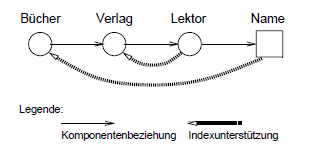
\includegraphics[scale=0.7]{img/index_legend.png}
			\end{figure}
			\begin{enumerate}
				\item Pfadindex\\
				verallgemeinert geschachtelter Index
				\begin{figure}[!h]
					\centering
					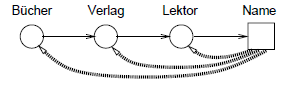
\includegraphics[scale=0.7]{img/path_index.png}
				\end{figure}
				\item Multiindex\\
				binäre Indexdateien von n-ter Komponenten des Pfadausdrucks auf (n-1)-te Komponente
				\begin{figure}[!h]
					\centering
					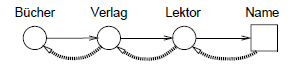
\includegraphics[scale=0.7]{img/multi_index.png}
				\end{figure}
				\item Verbundindex\\
				symmetrischer Multiindex
				\begin{figure}[!h]
					\centering
					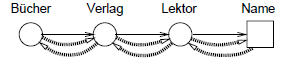
\includegraphics[scale=0.7]{img/join_index.png}
				\end{figure}
				\item geschachtelter Index\\
				eine einzige Indexdatei für n-te und erste Komponente des Pfadausdrucks
				\begin{figure}[!h]
					\centering
					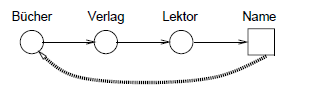
\includegraphics[scale=0.7]{img/nested_index.png}
				\end{figure}
				\item Zugriffsunterstützungsrelation (access support relation, ASR)\\
				Verallgemeinerung aller bisheriger Zugriffspfade, etwa verallgemeinerter (kompakter) Pfadindex
				\begin{figure}[!h]
					\centering
					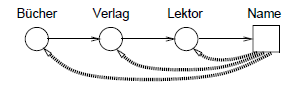
\includegraphics[scale=0.7]{img/asr_index.png}
				\end{figure}
			\end{enumerate}
		\end{itemize}
		\item \textbf{Zugriffspfade für Methoden}
		\begin{itemize}
			\item Ergebnisse der Methodenausführung im Index gespeichert
			\begin{itemize}
				\item parameterlose Methode: ein Methodenergebnis pro Objekt im Index\\
				\textit{eager:} bei Erzeugen/Ändern des Zustandes eines Objektes sofort Indexwert für Methodenergebnis berechnen und eintragen\\
				\textit{lazy:} beim ersten Aufruf der Methode für entsprechendes Objekt Indexwert für Methodenergebnis berechnen und eintragen
				
				\item parameterbehaftete Methode\\
				prinzipiell das Methodenergebnis pro Objekt und pro möglicher Parameterbelegung im Index speichern\\
				nicht effizient, also entweder nur bestimmte Bereiche aus der mgl Wertemenge in den Index\\
				oder nur Parameter in den Index, die schon einmal bei einer Anfrage benutzt wurden (lazy; adaptiver; lernender Index)
			\end{itemize}
			
			\item Materialisierung von Methodenergebnissen: Function-Materialization-Technik
		\end{itemize}
	\end{itemize}
	\item \textbf{Objektpuffer}
	\begin{itemize}
		\item bisher (RDBMS): Anwendungsdaten vom Seitenpuffer (komplett pder in das für Anwendungsprogramm verträglichen Teilen) in die Hauptspeicherbereiche laden, die dem Anwendungsprogramm zur Verfügung stehen
		\item kostet eine Transformation der internen Darstellung in die vom Anwendungsprogramm gewünschte
		\item in einigen System die Objekte von der Platte direkt in den Anwendungsspeicher: evtl mit gewissen Adresstransformationen
		\item andere OODBS haben zweiten Puffer: Objektpuffer
	\end{itemize}
	
	\item \textbf{Pointer Swizzling}
	\begin{itemize}
		\item ein im Hauptspeicher befindliches Objekt beim Zugriff aus dem Anwendungsprogramm heraus schnell finden
		\item mit Objektpuffer und logischen Objektidentitäten
		\begin{itemize}
			\item Objekt $\alpha$ im Hauptspeicher mit Kompontenobjekt $\beta$, das im Objektpuffer nicht gefunden wird
			\item Objekt $\beta$ im Seitenpuffer suchen => Seitenzuordnungstabelle (Resident Objet Table, ROT) durchmustern
			\item Falls $\beta$ nicht im Seiten puffer: vom Sekundärspeicher nachladen => Blockzuordnungstabelle (Persistent Object Table, POT) durchsuchen, um zu Objektidentität die Sekundärspeicheradresse zu ermitteln
			\item Nach Laden des Objektes in Seiten- und Objektpuffer müsste System aber bei jedem (!) $\beta$-Zugriff aus Anwendungsprogramm wiederum über logische Objektidentität die zugehörige Hauptspeicheradresse finden
		\end{itemize}
		\item zu umständliche und indirekt
		\item direkte Referenzen zur Implementierung der Objektidentität: eine Indirektion entfällt, aber im Hauptspeicher nützt die direkt (Sekundärspeicher-)Adresse nichts (muss auch gewandelt werden)
		\item Wegfall Objektpuffer: Transofmrtaion aus Seitenpuffer entfällt. Für Objekte im Seitenpuffer aber ebenfalls Hauptspeicheradressen zu berechnen
		\item Ziel: bei mehrfachen Zugriff auf im Hauptspeicher befindliche Objekte diese schneller finden => Transformation von indirekten oder direkten (Sekundärspeicher-) Referenzen in Hauptspeicheradressen (Pointer Swizzling)
		\item Original oder Kopie: Zeigertransformation auf Originalseite (im Seitenpuffer) oder auf Kopie (im Objektpuffer)? Systeme ohne Objektpuffer haben keine Wahl
		\item Sofort oder verzögert: Zeiger beim Laden transformieren oder verzögert beim ersten Zugriff auf das Objekt im Hauptspeicher?
		\item Direkt oder indirekt: Transformation in die direkte Hauptspeicheradresse durchgeführt oder nur in einen Deskriptor (indirekte Zeiger), der die Hauptspeicheradresse enthält
		\item heute bei main memory database systems
	\end{itemize}
\end{itemize}


\subsection{Transaktionen und Versionen}
\begin{itemize}
	\item Klassisch: Flache ACID-Transaktionen; OO:
	\begin{itemize}
		\item bestehen aus Teiltransaktionen
		\item Atomarität problematisch: ganz oder gar nicht am Ende einer wochenlangen Transaktionen?
		\item Isoliertheit problematisch (cooperative design im CAD; Weitergabe von inkonsistenten Objekten)
	\end{itemize}
	\item Objektorientierte Transaktionskonzepte\\
	ACID und mehr Struktur (geschachtelte Transaktionen)\\
	ACID aufgeben (lange Transaktionen; Sagas; Workflows)
	\begin{itemize}
		\item Lange Transaktionen
		\begin{itemize}
			\item CheckOut aus der DB in lokalen Arbeitsbereich ($T_1)$
			\item Objekt $o$ in DB nicht gesperrt
			\item andere Transaktion $T_2$ gibt vorher CheckIn von $o$ 
			\item CheckIn von $o$ durch $T_1$:\\
			schlägt fehl (GemStone)\\
			legt zwei Versionen an (ObjectStore)
		\end{itemize}
		\item Geschachtelte Transaktionen\\
		besteht aus Teiltransaktionen\\
		\textit{geschlossen:} alle UNLOCKs erst am Ende der Wurzeltransaktion\\
		\textit{offen:} UNLOCK nach jeder Teiltransaktion (unabhängige Komponenten, etwa Verlage)
		\begin{itemize}
			\item 
		\end{itemize}

	
		\item \textbf{ODMG-Transaktionen}
		\begin{itemize}
			\item ACID-Transaktionen und verteilte Transaktionen 
			\item transiente Objekte unterliegen nicht Transaktionskontrolle
			\item Sperren von Objekten Standard, Sperren von Seiten optional
			\item Sperren nach READ-WRITE-Modell
			\item Schnittstelle Transaction:
			\begin{itemize}
				\item begin() für den Start einer Transaktion
				\item commit() für das erfolgreiche Ende einer Transaktion
				\item abort() für den Abbruch einer Transaktion
				\item checkpoint() für die Synchronisation laufender Transaktionen, um einen konsistenten Zustand im Log-Protokoll zu erreichen
				\item active() zum Test auf eine aktive Transaktion
			\end{itemize}
			\item Schnittstelle Database Administrationsfunktionen:\\
			open, close(), bind, lookup für Datenbanken\\
			optional move, copy, reorganize, backup, restore für die Datensicherung
			
			\item geschachtelte Transaktionen in alten Versionen des Standards enthalten, ab ODMG 2.0 entfernt
		\end{itemize}
		
		\item \textbf{Erweiterte Transaktionsmodelle}
		\begin{itemize}
			\item Prinzipien anhand zweier Modelle:
			\item Geschachtelte Transaktionen: hierarchische Ansammlung von Vater-Sohn-Transaktionen
			\item Sagas: Zwischenergebnisse bereits durch ein Commit anderen Transaktionen verfügbar, aber trotzdem bei einem späteren Abbruch wieder rückgängig machen
			\item Transaktionsbaum und ihre ACID-Eigenschaften
			\begin{figure}[!h]
				\centering
				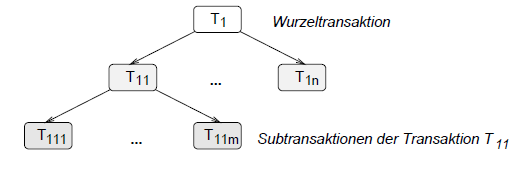
\includegraphics[scale=0.7]{img/transaction_tree.png}
			\end{figure}\\
			\textit{Isolation:} Ergebnisse einer Subtransaktion an die Vatertransaktion weitergeleitet, nicht sichtbar für andere nebenläufige Transaktionen\\
			\textit{Atomarität:} entweder alle Transaktionen des Transaktionsbaums enden erfolgreich oder brechen gemeinsam ab
		\end{itemize}
		
		\item \textbf{Geschlossen geschachtelte Transaktionen (CNT)}
		\begin{itemize}
			\item \textbf{Isolation:}
			\begin{itemize}
				\item Weitergabe der Sperren einer Subtransaktion an die Vatertransaktion, Sperren werden also in der Hierarchie nach oben (in Richtung der Wurzel) weitergereicht
				\item Ergebnisse der CNT werden erst mit dem Commit der Wurzeltransaktion freigegeben (ACID auf Wurzelebene)
			\end{itemize}
			\item \textbf{Atomarität}:
			\begin{enumerate}
				\item Abbruch einer Vatertransaktion erzwingt Abbruch aller Subtransaktionen
				\item Transaktion des Transaktionsbaumes kann nur erfolgreich enden, wenn alle Subtransaktionen erfolgreich waren
				\item Abbruch einer Subtransaktion führt zum Abbruch der Vatertransaktion
			\end{enumerate}
		\end{itemize}
		
		\item \textbf{Offen Geschachtelte Transaktionen (ONT)}
		\begin{itemize}
			\item keine Isolation: Ergebnisse werden bereits bei Commit der Subtransaktion freigegeben
			\item Atomarität offen geschachtelter Transaktionen\\
			geg: zwei Transaktionen $T_i, T_j$, wobein $T_j$ SOhn von $T_i$ ist\\
			ein abort($T_i$) erzwingt einen abort ($T_j$)\\
			ein commit($T_i$)  ist nur mgl nach einem commit($T_j$)
			
			\item Klassen von Subtransaktionen: vitale/nicht-vitale Transaktionen, Ersatztransaktionen
		\end{itemize}
		
		\item \textbf{Vitalität von Transaktionen}
		\begin{itemize}
			\item Vitalitätsbeziehung: Abbruch einer Transaktion führt zu Abbruch einer anderen Transaktion
			\item CNT: Abbruch der Subtransaktionen führt zum Abbruch der Vatertransaktion => Subtransaktion vital für Vatertransaktion
			\item CNT: Abbruch der Vatertransaktion führt zu Abbruch Subtransaktionen => Vatertransaktion vital für Subtransaktionen
			\item ONT: Abbruch Subtransaktion führt nicht zum Abbruch Vatertransaktion (ignore, s.u.) => Subtransaktion nicht-vital für Vatertransaktion
		\end{itemize}
		
		\item \textbf{ONT: Reaktion bei abort($T_j$)}
		\begin{enumerate}
			\item ignorieren (ignore) für nicht lebenswichtige (nicht-vitale) Subtransaktionen 
			\item erneutes Starten der abgebrochenen Subtransaktion: retry($T_j$), evtl. in Abhängigkeit von der Ursache des Abbruchs
			\item Versuch der Ausführung (try) einer Ersatztransaktion (contigency transaction)\\
			Ersatztransaktionen werden im Falle eines Abbruchs oder der Nichtausführbarkeit einer Transaktion alternativ ausgeführt.
			\item Abbruch des Vaters: abort($T_i$)
		\end{enumerate}
		Eigenschafte:\\
		\textit{Atomarität:} nur mit retry abgebrochener Subtransaktionen oder mit vitalen Subtransaktionen\\
		\textit{keine Atomariät:} bei nicht-vitalen Subtransaktionen und Ersatztransaktionen
		
		\item \textbf{Sagas}
		\begin{itemize}
			\item Bestandteile einer Saga:\\
			eine Menge von Transaktionen $T$\\
			für jede Transaktion $T_i \in T$ eine kompensierende Transaktion $C_i$, die den Zustand vor der Transaktion $T_i$ semantisch rückgängig macht.
			\item Saga = spezielle ONT der Tiefe 1
			\item keine Isolation: einzelne Subtransaktionen geben bei ihrem Commit Ergebnisse frei
			\item \textbf{Erlaubte Ausführungshistorien einer Saga}
			\begin{itemize}
				\item korrekte Ausführung: $T_1, \ldots, T_n$
				\item kontrollierter Abbruch: $T_1, \ldots, T_iC_iC_{i-1},\ldots, C_1$
				\item der zweite Fall tritt ein, wenn die Subtransaktion $T_{+1}, 1 \leq i < n$, abgebrochen wurde
				\item dann werden die Auswirkungen der Transaktionen $T_1$ bis $T_i$ mit Hilfe der Kompensationstransaktionen in umgekehrter Reihenfolge rückgängig gemacht
			\end{itemize}
			\item \textbf{Beispiel für ABlauf einer Saga}
			\begin{enumerate}
				\item Transaktion $T_1$: Hebe 10 Euro ab
				\item Transaktion $T_2$: Kaufe Gegenstand
				\item abort von $T_2$
				\item Kompensierende Transaktion $C_1$: Zahle 10 Euro ein
			\end{enumerate}
			\item Saga Modell bietet zwar keine Isolation, aber erfüllt D (durability) und A (atomicity)
		\end{itemize}
		
		\item \textbf{Entkoppelte SUbtransaktionen}
		\begin{itemize}
			\item ohne Wurzeltransaktion als Klammer
			\begin{figure}[!h]
				\centering
				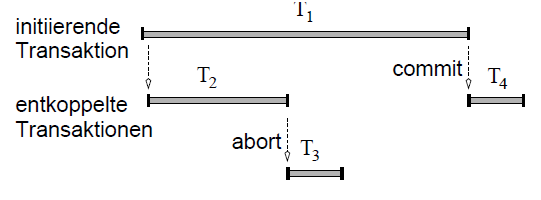
\includegraphics[scale=0.7]{img/root_transaction.png}
			\end{figure}
			\item Subtransaktionen können außerhalb des zeitlichen Rahmens der Wurzeltransaktionen laufen
			\item Eine Subtransaktion kann ein Commit machen, auch wenn die Vatertransaktion abbricht (Vatertransaktion nicht-vital für Subtransaktion)
			\item Neben dem expliziten Aufruf einer Subtransaktion kann eine Subtransaktion auch durch das Commit oder Abort einer anderen Transaktion aktiviert werden
			\item Entspricht Spezialfällen des Regelmodus detached but causally dependent in aktiven Datenbanken
			\item spezielle Abhängigkeiten sind parallel, sequential (Start der Transaktion nach erfolgreichem Ende der triggernden Transaktion) und exclusive (Start nur nach dem Abbruch der triggernden Transaktion)
		\end{itemize}
		
		\item \textbf{Von Transaktionen zu Workflows}
		\begin{itemize}
			\item Schritte ($S_i$) (ACID)
			\item ACID-Transaktionen ($T_j$)
			\item Arbeitsabläufe (Script): Sequenz, Verzweigung, Schleife, Parallelität
			\item ConTract:Workflow-Programmiermodell mit
			\item Schritten, Transaktionen, Scripts
			\item Programmiermodell mit Persistenz, Konsistenz, Recovery, Synchronisation, Kooperation
			\item Kompensation muss per Hand formuliert werden
			
			\begin{figure}[!h]
				\centering
				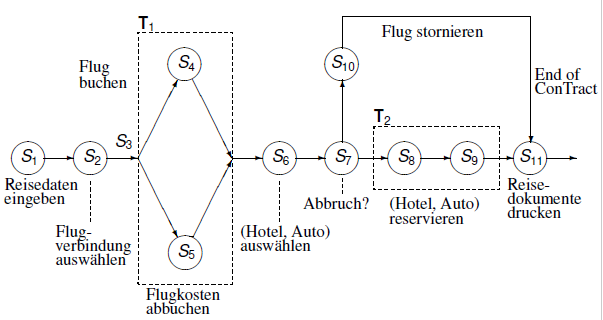
\includegraphics[scale=0.7]{img/contract_ex.png}
			\end{figure}
		\end{itemize}
		
		\item \textbf{Formalisierung von Inter-Transaktions-Beziehungen}
		\begin{itemize}
			\item Eigenschaften von erweiterten Transaktionsmodellen:
			\item Sichtbarkeit der Transaktionsergebnisse: offen vs. geschlossen
			\item Abbruchabhängigkeit der Vater- und Subtransaktionen: vital vs. nicht-vital
			\item Ausführungsreihenfolge von Subtransaktionen: parallel vs. sequentiell
		\end{itemize}
	\end{itemize}
		
	\item \textbf{Versionen und Konfigurationen}
	\begin{itemize}
		\item speziell für CASE; CAD; CIM wichtig: viele Versionen eines Objektes verwalten
		\item Erzeugung: explizit durch Benutzer; implizit durch System
		\item Verwaltung: Verzweigen, Zusammenführen, Löschen, Defaultversion wählen
		\item Konfigurationen\\
		falls Komponentenobjekte versioniert sind\\
		welche Komponentenversion gehört zu welcher Objektversion
	\end{itemize}
\end{itemize}


\subsection{Fazit, Rückblick, Ausblick}
\begin{itemize}
	\item \textbf{Rückblick (vor 13 Jahren)}\\
	Vorteile OODBMS
	\begin{itemize}
		\item OO pur nur im DB-Modell
		\item kein impedance mismatch bei oo Anwendungsprogrammierung
		\item Systeme nicht überladen
		\item Performance bei anfragelastigen Anwendungen sehr gut
	\end{itemize}
	Nachteile OODBMS
	\begin{itemize}
		\item schwacher, inkonsistenter Industriestandard
		\item DBMS-Funktionalitäten teilweise nicht enthalten\\
		Integritätssubsystem; Rechtevergabe; ONT, CNT, Sagas, kooperative Transaktionen; Datenunabhängigkeit fehlt, oft low-level Programmierung; Sichten
		\item Modellierung: Typsystem einer Programmiersprache ist kein DB-Modell
		\item Performance bei hoher Transaktionslast mit ACID-Anforderungen
	\end{itemize}
	
	\item \textbf{Stand 2015}
	\begin{itemize}
		\item OODMBS: Produkt für die Nische\\
		Std im Wesentlichen der Nachfolger des ODMG-Java-Binding: JDO\\
		ansonsten eher O-R-Mapper mit JPA\\
		leider keine Updates für ODMG/JDO
		
		\item ORDBMS: mit Oracle und DB2 weit verbreitet, wenn auch jeweils mit Einschränkungen:\\
		Std-SQL:1999/2003 bieten alle Konzepte der OO (ohne Mehrfachvererbung)
		\item SQL:"006 wird SQL/XML definieren: XML als Hype ab 2002\\
		für Multimedia-Dokumente flexibler als OO
	\end{itemize}
\end{itemize}